\section{Geometría dinámica}
\label{walls_holes}
Uno de los principales requerimientos para un planificador es la visualización de paredes y configuración de estas para adaptarlas a las medidas de una estancia. Además, deben poderse ubicar ventanas y puertas en las paredes, lo cual afecta a la geometría de la pared dado que se debe poder ver a través de estos elementos. Para ello no es factible utilizar mallas pregeneradas, se necesita generar las paredes de forma dinámica. También se han implementado techos y suelos con mallas dinámicas, pero el algoritmo para generar sus mallas proviene de un código del que ya se disponía antes de comenzar el proyecto, por lo que no se explicará.

En este apartado se describe el proceso de desarrollo de las paredes en 2 iteraciones, una primera en la que se crea una estructura básica para las paredes, y otra en la que se tienen en cuenta las ventanas y puertas.

%%%%%%%%%%%%%%%%%%%%%%%%%%%%%%%%%%%%%%%%%%%%%%%%%%%%%%%%%%%%%%%%%%%%%%%%%%%%%
%%%%%%%%%%%%%%%%%%%%%%%%%%%%%%%%%%%%%%%%%%%%%%%%%%%%%%%%%%%%%%%%%%%%%%%%%%%%%
%%%%%%%%%%%%%%%%%%%%%%%%%%%%%%%%%%%%%%%%%%%%%%%%%%%%%%%%%%%%%%%%%%%%%%%%%%%%%
\subsection{Generación de la estructura básica de la pared}
\label{subsec:gen1}
Por cada pared hay tres primeros puntos 2D relevantes: las esquinas izquierda de las paredes anterior, actual, y siguiente. A partir de estos tres puntos puede deducirse la información de la figura \ref{fig:wall_vectors}, donde los vectores ``N1" y ``N2" son las normales de cada pared, siempre hacia el exterior de la estancia.

\begin{figure}[H]
    \centering
    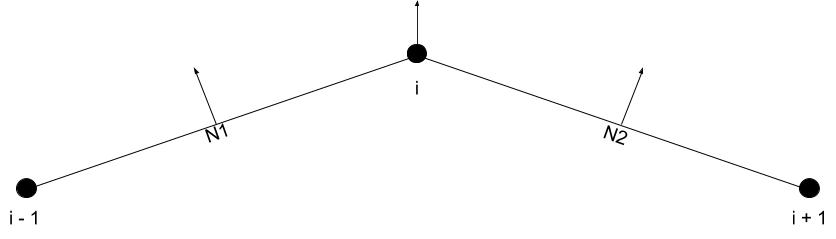
\includegraphics[width=\linewidth]{data_from_3_points}
    \caption{Vectores extraídos a partir de 3 puntos consecutivos.}
    \label{fig:wall_vectors}
\end{figure}

``N1" y ``N2" pueden obtenerse normalizando los vectores de un punto a otro, y girándolos. La dirección del vector central es la suma normalizada de estos dos o, en el caso de las paredes en los extremos cuando el circuito no está cerrado, la normal de la propia pared:

\begin{lstlisting}
OBTENER INDICES DE PARED actual, anterior Y siguiente

v_pc = puntos[actual] - puntos[anterior];
v_cn = puntos[siguiente] - puntos[actual];

SI cerrado Y actual ES LA PRIMERA O ULTIMA PARED ENTONCES:
    normal_actual = GIRAR 90 GRADOS ANTI-HORARIO v_cn Y NORMALIZAR
    direccion = puntos[actual] + normal_actual
SINO
    normal_actual = GIRAR 90 GRADOS ANTI-HORARIO v_cn
    normal_anterior = GIRAR 90 GRADOS ANTI-HORARIO v_pc
    direccion = normal_actual + normal_anterior
    NORMALIZAR direccion
FINSI
\end{lstlisting}

Por último se debe tener en cuenta el grosor que se espera que tenga la pared, dado que si se avanza siempre la misma distancia en el vector director el grosor de estas dependería del ángulo que formen con sus paredes adyacentes. Esto se resuelve con trigonometría:

\begin{lstlisting}
SI cerrado ENTONCES:
    direccion = profundidad_pared / absoluto(producto_punto(normal_actual, direccion));
SINO
    direccion = profundidad_pared * normal_actual
FINSI

punto_esquina = puntos[actual] + direccion
\end{lstlisting}

El producto punto de dos vectores normales es el coseno del ángulo que forman entre sí. En este momento ``direccion" incluye la dirección y distancia entre el punto actual y el punto de la esquina exterior, permitiendo generar dicho punto a partir del actual. En el caso de que la pared que estamos generando no haga esquina con otra, simplemente se utiliza la normal de la pared actual.

Una limitación de este sistema es que los puntos deben introducirse en sentido anti-horario respecto al interior de la habitación. De lo contrario la normal de cada pared queda invertida y estas se extienden hacia el lado opuesto al que deberían, provocando algunos artefactos no deseados.

%%%%%%%%%%%%%%%%%%%%%%%%%%%%%%%%%%%%%%%%%%%%%%%%%%%%%%%%%%%%%%%%%%%%%%%%%%%%%
%%%%%%%%%%%%%%%%%%%%%%%%%%%%%%%%%%%%%%%%%%%%%%%%%%%%%%%%%%%%%%%%%%%%%%%%%%%%%
%%%%%%%%%%%%%%%%%%%%%%%%%%%%%%%%%%%%%%%%%%%%%%%%%%%%%%%%%%%%%%%%%%%%%%%%%%%%%
\subsection{Índices para la estructura básica}
La pared tiene 23 vértices y no 8 como cabría esperar. Esto se debe a que al renderizar, los shaders interpolan la normal de cada vértice con la de sus vecinos; si el mismo vértice se encuentra en dos caras distintas, la normal del vértice no coincide con la de la superficie en la cara que se está pintando. El resultado de esto sería que el color varía en los bordes de cada cara. Esta propiedad es muy útil para objetos que no tienen ángulos tan marcados, pero en este caso se busca que las caras sean muy marcadas y totalmente planas.

Para solucionarlo se repite cada vértice tantas veces como el número de caras en el que se encuentre, de modo que aunque todos se encuentren en la misma posición, cada cara está utilizando un vértice distinto.

\begin{figure}[H]
    \centering
    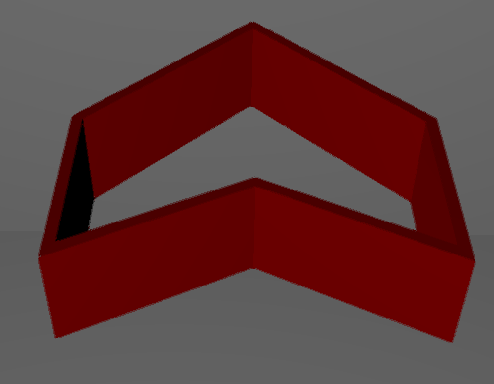
\includegraphics[width=0.55\linewidth]{paredes_first}
    \caption{Ejemplo de generación de paredes.}
    \label{fig:paredes_first}
\end{figure}

%%%%%%%%%%%%%%%%%%%%%%%%%%%%%%%%%%%%%%%%%%%%%%%%%%%%%%%%%%%%%%%%%%%%%%%%%%%%%
%%%%%%%%%%%%%%%%%%%%%%%%%%%%%%%%%%%%%%%%%%%%%%%%%%%%%%%%%%%%%%%%%%%%%%%%%%%%%
%%%%%%%%%%%%%%%%%%%%%%%%%%%%%%%%%%%%%%%%%%%%%%%%%%%%%%%%%%%%%%%%%%%%%%%%%%%%%
\subsection{Modificando la estructura para permitir la inclusión de ventanas}
\label{subsec:gen2}
Como se puede ver en el apartado de diseño (\ref{holes_design}) se requiere modificar la geometría para que el lado anterior y posterior de las paredes sean idénticos. Esto, sin embargo, complica las conexiones entre los vértices, que se han tenido que generar manualmente. Con los nuevos vértices añadidos en total hay 35 vértices.

\begin{figure}[H]
    \centering
    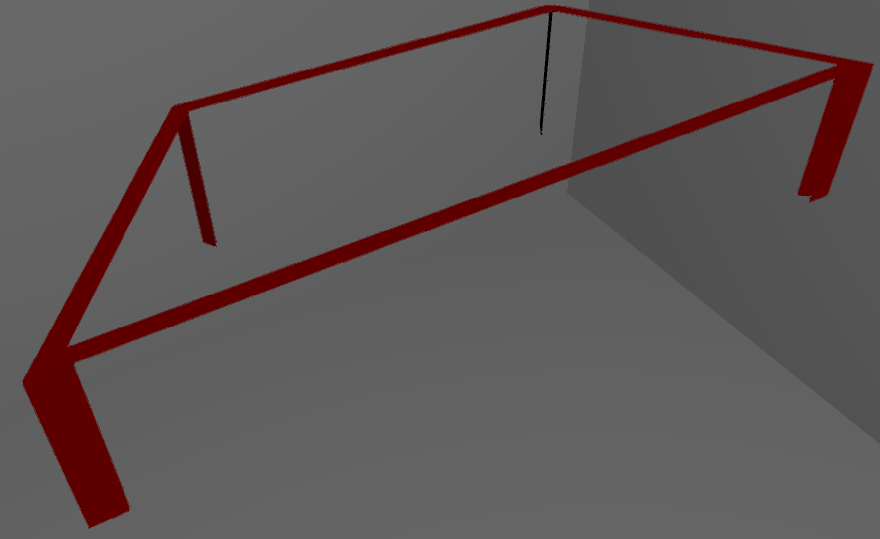
\includegraphics[width=0.75\linewidth]{paredes_frame}
    \caption{Aspecto de las paredes sin los planos anterior y posterior.}
    \label{fig:nueva_estructura}
\end{figure}

En la figura \ref{fig:nueva_estructura} puede verse el resultado. Nótese que los planos inferiores no se ven porque sus normales apuntan hacia abajo y el motor gráfico los oculta como optimización. Al crear los índices se ha tenido en cuenta el orden de estos, pues afecta al cálculo de las normales de los vértices.

%%%%%%%%%%%%%%%%%%%%%%%%%%%%%%%%%%%%%%%%%%%%%%%%%%%%%%%%%%%%%%%%%%%%%%%%%%%%%
%%%%%%%%%%%%%%%%%%%%%%%%%%%%%%%%%%%%%%%%%%%%%%%%%%%%%%%%%%%%%%%%%%%%%%%%%%%%%
%%%%%%%%%%%%%%%%%%%%%%%%%%%%%%%%%%%%%%%%%%%%%%%%%%%%%%%%%%%%%%%%%%%%%%%%%%%%%
%\clearpage
\subsection{Generación de ventanas I: proyección sobre pared}
\label{sec:wallgenwindowsi}
Como ya se ha mencionado en el apartado \ref{holes_design}, las ventanas están definidas por un punto, una altura y un ancho. No se incluye ninguna información respecto a que pared es la que va a contener dicha ventana; por lo que se cogerá la pared más cercana al punto dado.

Para ello se proyecta el punto sobre la línea $AB$ de cada una de las paredes, calculando la distacia hasta cada una de las proyecciones para ver cuál es la más cercana (véase el apéndice \ref{sec:pointrayproj} sobre la proyección punto-línea).

Como preparación para el próximo apartado (\ref{sec:wallgenwindowsii}) se calcula sobre la pared los 4 puntos que delimitarán la ventana. Para ello se proyecta el punto de la pared sobre el plano que forma esta, y se calcula el resto de puntos desplazándonos por dicho plano (véase el apéndice \ref{sec:pointplaneproj} sobre la proyección punto-rectángulo):

\begin{lstlisting}
projectVertices(pared, referencia a hueco):
    origen = PROYECTAR ORIGEN DEL HUECO SOBRE PLANO DE LA PARED
    
    hueco.A1 = origen
    hueco.B1 = origen + DIRECCION DERECHA * hueco.ancho
    hueco.A1H = origen + DIRECCION ARRIBA * hueco.alto
    hueco.B1H = hueco.A1H + DIRECCION DERECHA * hueco.ancho
FIN DE FUNCION
\end{lstlisting}

%%%%%%%%%%%%%%%%%%%%%%%%%%%%%%%%%%%%%%%%%%%%%%%%%%%%%%%%%%%%%%%%%%%%%%%%%%%%%
%%%%%%%%%%%%%%%%%%%%%%%%%%%%%%%%%%%%%%%%%%%%%%%%%%%%%%%%%%%%%%%%%%%%%%%%%%%%%
%%%%%%%%%%%%%%%%%%%%%%%%%%%%%%%%%%%%%%%%%%%%%%%%%%%%%%%%%%%%%%%%%%%%%%%%%%%%%
\subsection{Generación de ventanas II: modificación de la geometría de la pared}
\label{sec:wallgenwindowsii}

Al final del apartado \ref{sec:wallgenwindowsi}, ya se conoce el punto en que están los extremos de la ventana sobre la pared. En este apartado se explica cómo dividir la pared en diferentes planos y descartar aquellos que correspondan a un agujero.

Una vez más las proyecciones cobran mucho protagonismo (véase el apéndice \ref{sec:pointrayproj} sobre la proyección punto-línea). Lo primero que se busca es dividir el plano de la pared por los vértices del hueco, obteniendo una colección de planos.

El algoritmo para conseguir esto tiene como entrada y salida una lista de planos, que empieza siendo uno solo que cubre toda la pared. Mientras iteramos los puntos, proyectamos estos sobre cada lado para obtener los puntos por los que hay que cortar los planos, y posteriormente se añaden a la lista de planos desechando el original. En caso de que una de las proyecciones no contribuya a crear un nuevo plano (como por ejemplo, los puntos inferiores de la puerta en la figura \ref{fig:mult_and_red_windows}) la ignoramos.

Posteriormente se comprueba cuales de estos planos forman parte de una ventana y se eliminan de la lista, dejando un hueco en dicha posición. Este algoritmo permite además añadir múltiples ventanas, aumentando la posible complejidad de la pared.

Por último se reprocesan los planos generados comprobando si sus lados coinciden en alguna dirección, en cuyo caso se reúnen para reducir la complejidad. En la figura \ref{fig:mult_and_red_windows}, se puede ver un ejemplo de como se separan los planos con múltiples ventanas, y cómo se reúnen los planos adyacentes.

\begin{figure}[H]
    \centering
    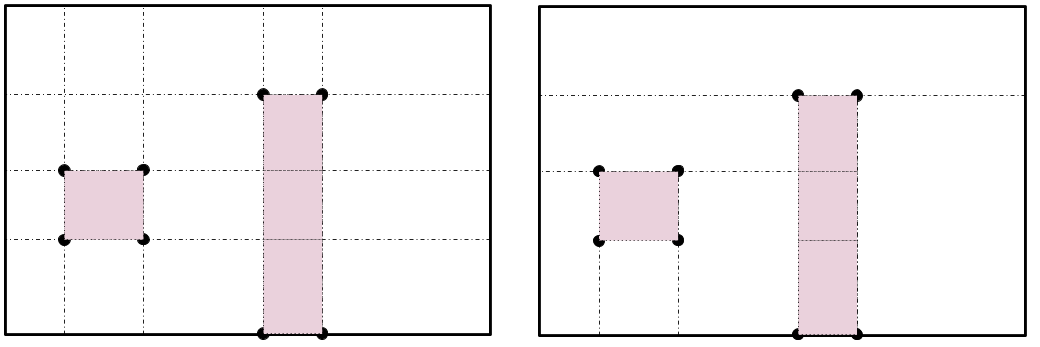
\includegraphics[width=0.85\linewidth]{mult_window_and_reduction}
    \caption{Ejemplo de pared con una ventana y una puerta, y muestra de una posible reducción de los planos.}
    \label{fig:mult_and_red_windows}
\end{figure}

\begin{figure}[H]
    \centering
    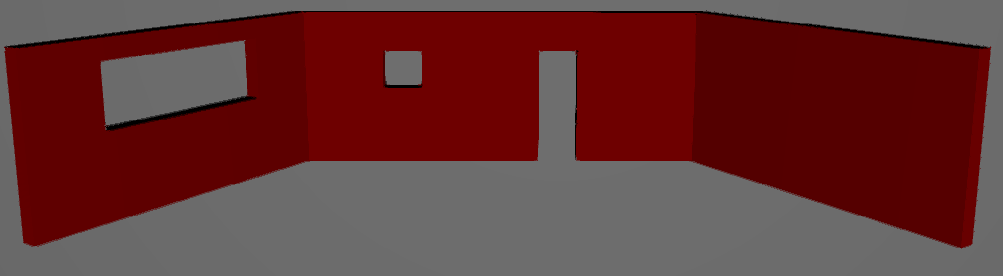
\includegraphics[width=0.85\linewidth]{Agujeros}
    \caption{Ejemplo de generación de paredes con huecos y estancia sin cerrar.}
    \label{fig:wall_with_window_example}
\end{figure}

%%%%%%%%%%%%%%%%%%%%%%%%%%%%%%%%%%%%%%%%%%%%%%%%%%%%%%%%%%%%%%%%%%%%%%%%%%%%%
%%%%%%%%%%%%%%%%%%%%%%%%%%%%%%%%%%%%%%%%%%%%%%%%%%%%%%%%%%%%%%%%%%%%%%%%%%%%%
%%%%%%%%%%%%%%%%%%%%%%%%%%%%%%%%%%%%%%%%%%%%%%%%%%%%%%%%%%%%%%%%%%%%%%%%%%%%%
\subsection{Generación de uvs}
Para que el motor aplique correctamente las texturas sobre las paredes, se requiere que las uvs estén a escala de mundo; es decir, se espera que dada una distancia entre dos vértices de la mima malla, sus uvs tengan la misma distancia. La mayor dificultad en este caso está en que los vértices se encuentran en espacio tridimensional, mientras que las uv son coordenadas bidimensionales de la textura que estamos mapeando. Por lo tanto, de algún modo hay que desconsiderar la orientación de la pared y centrarnos en sus superficies.

Como la geometría está formada por planos perfectos, la solución encontrada ha consistido en partir siempre de la esquina inferior izquierda de cada uno de ellos. Como precondición, la esquina ``A" tiene la uv (0,0).

Por lo tanto por cada plano, se ha definido la uv de la esquina inferior izquierda, y los vectores hacia los cuales ``avanzan" las componentes \texttt{x} e \texttt{y} de las uv (Fig. \ref{fig:datos_uvs}).

\begin{figure}[H]
    \centering
    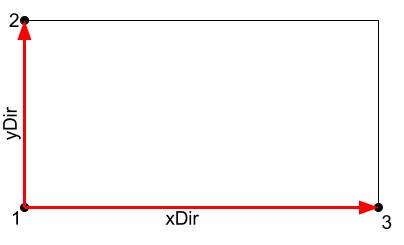
\includegraphics[scale=0.75]{Datos_uvs}
    \caption{Datos necesarios para la generación de las uv ``2" y ``3".}
    \label{fig:datos_uvs}
\end{figure}

La razón de usar proyecciones y no la magnitud de los vectores directamente, es que se desconoce en cual de las dos direcciones se encuentra el vértice que observamos al iterar. Proyectando cada punto tenemos la distancia en cada una de las dos direcciones y se la sumamos a la uv del vértice ``1":

\begin{lstlisting}
genUV(origen, xDir, yDir, punto, uv_origen, longitud_x, longitud_y):
    uv.x = PROYECTAR punto SOBRE RAYO EN DIRECCION xDir
    uv.y = PROYECTAR punto SOBRE RAYO EN DIRECCION yDir
    
    SI uv.x ES SUPERIOR A LA LONGITUD HORIZONTAL DE LA PARED ENTONCES:
        uv.x = longitud_x - uv.x
    FINSI
    SI uv.y ES SUPERIOR A LA LONGITUD VERTICAL DE LA PARED ENTONCES:
        uv.y = longitud_y - uv.y
    FINSI
    
    uv = uv + uv_origen
    DEVOLVER uv
FIN DE FUNCION
\end{lstlisting}

Dado que las uv no pueden ser negativas, se hace un paso en las líneas 6-11 para que, en caso de serlo, se les sume la longitud total del lado en el que se encuentran.

%%%%%%%%%%%%%%%%%%%%%%%%%%%%%%%%%%%%%%%%%%%%%%%%%%%%%%%%%%%%%%%%%%%%%%%%%%%%%
%%%%%%%%%%%%%%%%%%%%%%%%%%%%%%%%%%%%%%%%%%%%%%%%%%%%%%%%%%%%%%%%%%%%%%%%%%%%%
%%%%%%%%%%%%%%%%%%%%%%%%%%%%%%%%%%%%%%%%%%%%%%%%%%%%%%%%%%%%%%%%%%%%%%%%%%%%%
\subsection{Generación de normales, tangentes y bitangentes}
El cálculo de cada normal es el resultado de la suma de la normal de cada polígono en el que se encuentra dicho vértice, y para calcular esta se hace el producto vectorial (normalizado) de los vectores que van del primer vértice hacia el segundo y el tercero:

\begin{lstlisting}
DADOS LOS PUNTOS v1, v2 Y v3

normal = NORMALIZAR ( PRODUCTO CRUZADO DE (v2 - v1) Y (v3 - v1))
\end{lstlisting}

Las tangentes y bitangentes son un poco más complicadas: todo vector tiene infinitos vectores tangentes, pero en este caso no sirve cualquiera. El vector tangente a la normal tiene que estar siempre alineado con las uv.
\clearpage
Como se explica en el tutorial 13 de opengl-tutorial.org \footfullcite{opengltutorials}, para ello debemos resolver el siguiente sistema de ecuaciones:


\[ deltaPos1 = deltaUV1.x * T + deltaUV1.y * B \]
\[ deltaPos2 = deltaUV2.x * T + deltaUV2.y * B \]

Esto se computa del siguiente modo:

\begin{lstlisting}
DADOS TRES PUNTOS v1, v2 y v3
vec1 = v2 - v1
vec2 = v3 - v1

deltaUV1 = uv2 - uv1
deltaUV2 = uv3 - uv1

r = 1.0 / (deltaUV1.x * deltaUV2.y - deltaUV1.y * deltaUV2.x)

tangente = (vec1 * deltaUV2 - vec2 * deltaUV1.y) * r
bitangente = (vec2 * deltaUV1.x - vec1 * deltaUV2.x) * r
\end{lstlisting}

\begin{figure}[H]
    \centering
    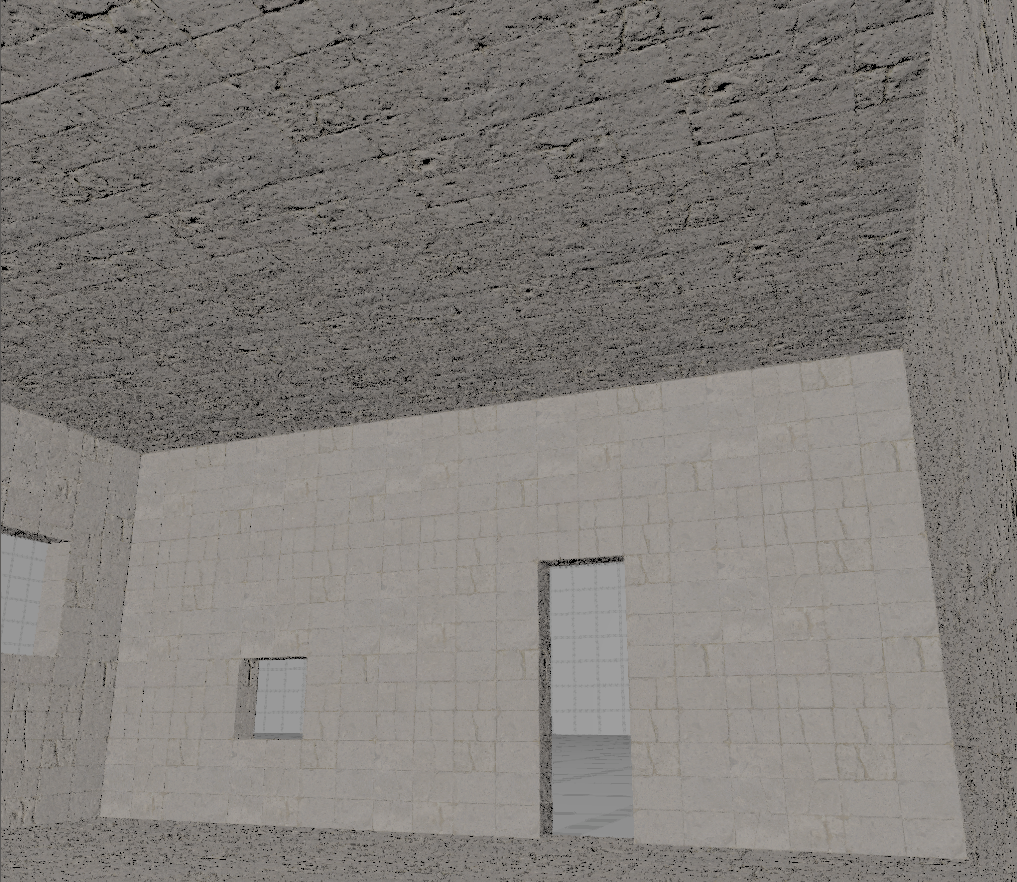
\includegraphics[width=0.75\linewidth]{paredes_uvs}
    \caption{Ejemplo de una habitación con texturas de prueba.}
    \label{fig:ejemplo_con_uvs}
\end{figure}
